\documentclass{beamer}

\usetheme {Madrid}

\usepackage{graphicx}     %Note graphics<graphicx<epsfig
\usepackage[table,xcdraw, dvipsnames]{xcolor}
\usepackage{hyperref} %written by Sebastian Rahtz
%\usepackage{subeqn}    %allows equations 1a, 1b
%\usepackage{subfig}    %allows figures 1a, 1b
\usepackage{amsmath}
\usepackage{amssymb}
\usepackage{xurl}
\usepackage{bbm}%for indicator function
%\bibliographystyle{alpha}
\usepackage{floatrow}
\usepackage[normalem]{ulem}
\usepackage{tikz}
\usepackage{xparse, expl3, istgame, makecell}

\usepackage[color,matrix,frame,arrow,curve]{xy}
\newcommand{\rv}[1]{{\,\ul{#1}\,}}

\newcommand{\bra}[1]{\langle#1|}
\newcommand{\ket}[1]{|#1\rangle}
\newcommand{\av}[1]{\left\langle#1\right\rangle}
\newcommand{\pder}[2]{\frac{\partial#1}{\partial#2}}
\newcommand{\der}[2]{\frac{d#1}{d#2}}
\newcommand{\tr}[0]{{\rm tr }}
\newcommand{\beq}{\begin{equation}}
\newcommand{\eeq}{\end{equation}}
\newcommand{\bsub}{\begin{subequations}}
	\newcommand{\esub}{\end{subequations}}
\newcommand{\beqa}{\begin{eqnarray}}
\newcommand{\eeqa}{\end{eqnarray}}
\newcommand{\rarrow}[0]{\rightarrow}
\newcommand{\larrow}[0]{\leftarrow}
\newcommand{\uarrow}[0]{\uparrow}
\newcommand{\darrow}[0]{\downarrow}
\newcommand{\Rarrow}[0]{\Rightarrow}
\newcommand{\nRarrow}[0]{\nRightarrow}
\newcommand{\Larrow}[0]{\Leftarrow}
\newcommand{\nLarrow}[0]{\nLeftarrow}
\newcommand{\ul}[1]{\uline{#1}}
\newcommand{\ol}[1]{\overline{#1}}
\newcommand{\CC}[0]{{ \mathbb{C}} }
\newcommand{\EE}[0]{{ \mathbb{E}} }
\newcommand{\NNN}[0]{ {\mathbb{N}}} %\NN already defined
\newcommand{\PP}[0]{{ \mathbb{P}} }
\newcommand{\RR}[0]{{ \mathbb{R}} }
\newcommand{\WW}[0]{ {\mathbb{W}}}
\newcommand{\XX}[0]{{ \mathbb{X}} }
\newcommand{\YY}[0]{{ \mathbb{Y}} }
\newcommand{\ZZ}[0]{ {\mathbb{Z}}}

\renewcommand{\Re}{{\rm Re}}
\renewcommand{\Im}{{\rm Im}}



\newcommand{\ground}{{}_{\stackrel{\stackrel{\displaystyle{\bot}}{-}}{.}}}
\newcommand{\norm}[1]{\parallel#1\parallel}
\newcommand{\eqdef}[0]{\;\;\stackrel{\text{def}}{=}\;\;}

\newcommand{\heavy}[0]{\mathbf{H}}

\newcommand{\rva}[0]{{\ul{a}}}
\newcommand{\rvb}[0]{{\ul{b}}}
\newcommand{\rvc}[0]{{\ul{c}}}
\newcommand{\rvd}[0]{{\ul{d}}}
\newcommand{\rve}[0]{{\ul{e}}}
\newcommand{\rvf}[0]{{\ul{f}}}
\newcommand{\rvg}[0]{{\ul{g}}}
\newcommand{\rvh}[0]{{\ul{h}}}
\newcommand{\rvi}[0]{{\ul{i}}}
\newcommand{\rvj}[0]{{\ul{j}}}
\newcommand{\rvk}[0]{{\ul{k}}}
\newcommand{\rvl}[0]{{\ul{l}}}
\newcommand{\rvll}[0]{{\ul{\ell}}}
\newcommand{\rvm}[0]{{\ul{m}}}
\newcommand{\rvn}[0]{{\ul{n}}}
\newcommand{\rvo}[0]{{\ul{o}}}
\newcommand{\rvp}[0]{{\ul{p}}}
\newcommand{\rvq}[0]{{\ul{q}}}
\newcommand{\rvr}[0]{{\ul{r}}}
\newcommand{\rvs}[0]{{\ul{s}}}
\newcommand{\rvt}[0]{{\ul{t}}}
\newcommand{\rvu}[0]{{\ul{u}}}
\newcommand{\rvv}[0]{{\ul{v}}}
\newcommand{\rvw}[0]{{\ul{w}}}
\newcommand{\rvx}[0]{{\ul{x}}}
\newcommand{\rvy}[0]{{\ul{y}}}
\newcommand{\rvz}[0]{{\ul{z}}}


\newcommand{\rvA}[0]{{\ul{A}}}
\newcommand{\rvB}[0]{{\ul{B}}}
\newcommand{\rvC}[0]{{\ul{C}}}
\newcommand{\rvD}[0]{{\ul{D}}}
\newcommand{\rvE}[0]{{\ul{E}}}
\newcommand{\rvF}[0]{{\ul{F}}}
\newcommand{\rvG}[0]{{\ul{G}}}
\newcommand{\rvH}[0]{{\ul{H}}}
\newcommand{\rvI}[0]{{\ul{I}}}
\newcommand{\rvJ}[0]{{\ul{J}}}
\newcommand{\rvK}[0]{{\ul{K}}}
\newcommand{\rvL}[0]{{\ul{L}}}
\newcommand{\rvM}[0]{{\ul{M}}}
\newcommand{\rvN}[0]{{\ul{N}}}
\newcommand{\rvO}[0]{{\ul{O}}}
\newcommand{\rvP}[0]{{\ul{P}}}
\newcommand{\rvQ}[0]{{\ul{Q}}}
\newcommand{\rvR}[0]{{\ul{R}}}
\newcommand{\rvS}[0]{{\ul{S}}}
\newcommand{\rvT}[0]{{\ul{T}}}
\newcommand{\rvU}[0]{{\ul{U}}}
\newcommand{\rvV}[0]{{\ul{V}}}
\newcommand{\rvW}[0]{{\ul{W}}}
\newcommand{\rvX}[0]{{\ul{X}}}
\newcommand{\rvY}[0]{{\ul{Y}}}
\newcommand{\rvZ}[0]{{\ul{Z}}}

\newcommand{\rvbeta}[0]{{\ul{\beta}}}
\newcommand{\rvxi}[0]{{\ul{\xi}}}
\newcommand{\rvzeta}[0]{{\ul{\zeta}}}
\newcommand{\rvtheta}[0]{{\ul{\theta}}}
\newcommand{\rvmu}[0]{{\ul{\mu}}}
\newcommand{\rvsig}[0]{{\ul{\sigma}}}
\newcommand{\rvDel}[0]{{\ul{\Delta}}}
\newcommand{\rvtau}[0]{{\ul{\tau}}}

\newcommand{\cala}[0]{{\cal A}}
\newcommand{\calb}[0]{{\cal B}}
\newcommand{\calc}[0]{{\cal C}}
\newcommand{\cald}[0]{{\cal D}}
\newcommand{\cale}[0]{{\cal E}}
\newcommand{\calf}[0]{{\cal F}}
\newcommand{\calg}[0]{{\cal G}}
\newcommand{\calh}[0]{{\cal H}}
\newcommand{\cali}[0]{{\cal I}}
\newcommand{\calk}[0]{{\cal K}}
\newcommand{\call}[0]{{\cal L}}
\newcommand{\calm}[0]{{\cal M}}
\newcommand{\caln}[0]{{\cal N}}
\newcommand{\calo}[0]{{\cal O}}
\newcommand{\calp}[0]{{\cal P}}
\newcommand{\calq}[0]{{\cal Q}}
\newcommand{\calr}[0]{{\cal R}}
\newcommand{\cals}[0]{{\cal S}}
\newcommand{\calt}[0]{{\cal T}}
\newcommand{\calu}[0]{{\cal U}}
\newcommand{\calv}[0]{{\cal V}}
\newcommand{\calw}[0]{{\cal W}}
\newcommand{\calx}[0]{{\cal X}}
\newcommand{\caly}[0]{{\cal Y}}
\newcommand{\calz}[0]{{\cal Z}}

%\newcommand{\diamante}[1]{\Big\langle#1\Big\rangle}
\newcommand{\diamante}[1]{*++[F=]{#1}}
%\newcommand{\corchete}[1]{\Big\{#1\Big\}}
\newcommand{\corchete}[1]{#1}
\newcommand{\cuadro}[1]{*++[F]{#1}}

\newcommand{\Pmat}[4]{\calp\left[
\begin{array}{cc}#1&#2\\#3&#4
\end{array}\right]}

%\newcommand{\PN}[0]{PN^{0,0}_{1,1}}
%\newcommand{\PS}[0]{PS^{1,1}_{0,0}}
\newcommand{\PN}[0]{PN}
\newcommand{\PS}[0]{PS}

\newcommand{\lam}[0]{\lambda}
\newcommand{\Lam}[0]{\Lambda}
\newcommand{\alp}[0]{\alpha}
\newcommand{\eps}[0]{\epsilon}
\newcommand{\s}[0]{\sigma}
\newcommand{\su}[0]{{\Sigma}}

\newcommand{\pp}[0]{\mathbb{P}}
\newcommand{\dbm}[0]{{
		[1,\partial_{b},\partial_{m}]
}}

\newcommand{\dg}[0]{{[1, \partial_{\theta_G}]}}
\newcommand{\dd}[0]{{[1, \partial_{\theta_D}]}}
\newcommand{\dgd}[0]{{[1, \partial_{\theta_G}, \partial_{\theta_D}]}}

\newcommand{\veca}[0]{{\vec{a}}}
\newcommand{\vecb}[0]{{\vec{b}}}
\newcommand{\vecc}[0]{{\vec{c}}}
\newcommand{\vecd}[0]{{\vec{d}}}
\newcommand{\vecf}[0]{{\vec{f}}}
\newcommand{\vech}[0]{{\vec{h}}}
\newcommand{\vecr}[0]{{\vec{r}}}
\newcommand{\vecs}[0]{{\vec{s}}}
\newcommand{\vecu}[0]{{\vec{u}}}
\newcommand{\vecx}[0]{{\vec{x}}}
\newcommand{\vecy}[0]{{\vec{y}}}
\newcommand{\vechy}[0]{{\vec{\haty}}}
\newcommand{\vtheta}[0]{{\vec{\theta}}}

\newcommand{\haty}[0]{{\widehat{y}}}
\newcommand{\hatx}[0]{{\widehat{x}}}
\newcommand{\hata}[0]{{\widehat{a}}}
\newcommand{\hatr}[0]{{\widehat{r}}}


\newcommand{\cond}[0]{{\:\mathbf{|}\:}}
\newcommand{\mymathbf}[1]{#1}

\newcommand{\ranvec}[1]{\ul{\vec{#1}}}
\newcommand{\indi}[0]{\mathbbm{1}}
\newcommand{\smoid}[0]{{\rm smoid}}
\newcommand{\lodds}[0]{{\rm lodds}}
\newcommand{\expit}[0]{{\rm expit}}
\newcommand{\logit}[0]{{\rm logit}}
\newcommand{\sign}[0]{{\rm sign}}

%\renewcommand{\labelitemii}{$\bullet$}

\newcommand{\HAT}[1]{{\widehat{#1}}}
\newcommand{\TIL}[1]{{\widetilde{#1}}}
\newcommand{\tild}[0]{{\TIL{d}}}
\newcommand{\tile}[0]{{\TIL{e}}}
\newcommand{\tilg}[0]{{\TIL{g}}}
\newcommand{\tilu}[0]{{\TIL{u}}}
\newcommand{\tilx}[0]{{\TIL{x}}}
\newcommand{\tilP}[0]{{\TIL{P}}}
\newcommand{\tilPT}[0]{{\TIL{P}_\theta}}

\newcommand{\maparrow}[1]
{\xymatrix{\ar[r]_{#1}&}}


\newcommand{\ucalm}[0]{\ul{\calm}}

\newcommand{\bool}[0]{\{0,1\}}

\newcommand{\argmin}{\mathop{\mathrm{argmin}}\limits}
\newcommand{\argmax}{\mathop{\mathrm{argmax}}\limits}

\newcommand{\softmax}[0]{{\rm softmax}}


\usepackage{wrapfig}
\newcommand{\BSframe}[1]{\begin{frame}
{#1}\section{#1}}
\newcommand{\BSSframe}[1]{\begin{frame}
{#1}\subsection{#1}}


%\definecolor{myred}{RGB}{153, 18, 2}
%\setbeamercolor{structure}{fg=myred}

\title{www.ar-tiste.xyz  Pitchdeck 2025}

\titlegraphic{
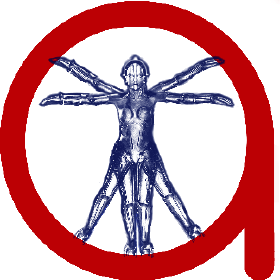
\includegraphics[width=3cm]{ar-tiste-logo.png}
}
\author{\href{www.ar-tiste.xyz}{www.ar-tiste.xyz}}

\begin{document}

\begin{frame}
\maketitle

\end{frame}

\begin{frame}[allowframebreaks]{Contents}
\tableofcontents
\end{frame}




\BSframe{Past: Distinguishing between correlation and causation}

\begin{wrapfigure}{l}{0.8\textwidth}
   \centering
    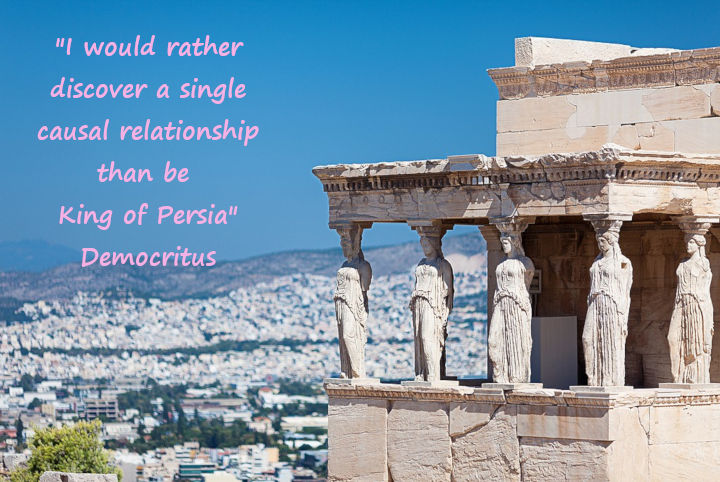
\includegraphics[width=0.8\textwidth]
    {democritus-acropolis-caryatids.jpg}

\end{wrapfigure}


Distinguishing between correlation and causation is necessary in all the sciences.
It is the goal of science and of the scientific method.


\end{frame}


\BSframe{Present: Clayton Christensen on Causality}

$$
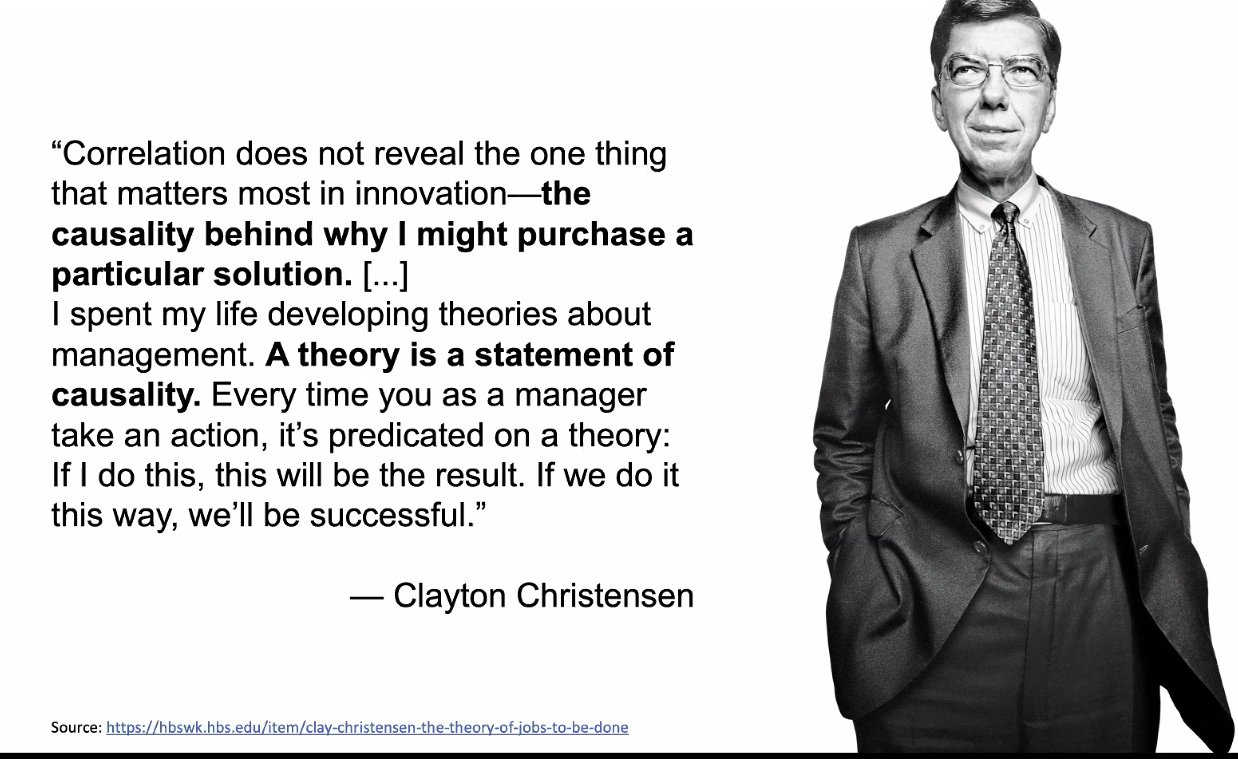
\includegraphics[width=.9\textwidth]{clayton-christensen-causality.jpeg}
$$

\end{frame}

\BSframe{Future: Spock-GPT}

$$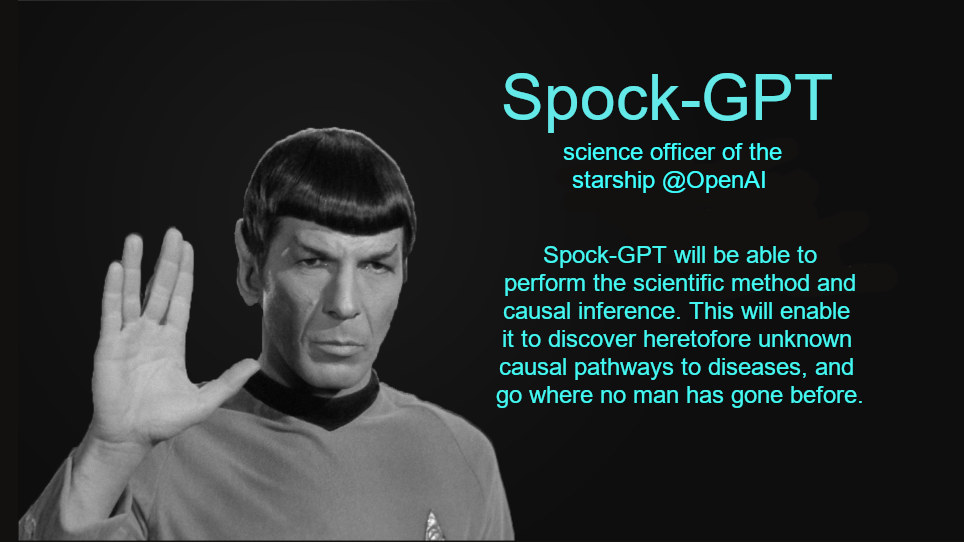
\includegraphics[width=.9\textwidth]{spock-gpt.jpg}$$

\end{frame}


\BSframe{What problems does ar-tiste.xyz solve?}

\begin{itemize}
    \item Healthcare and Biotech: finding causal pathways for diseases
    \item Business Management, A/B test and beyond
    \item Longevity research
    \item Dieting
    \item \ldots
\end{itemize}

\end{frame}

\BSframe{Startups applying causal AI to healthcare/biotech}

%\begin{itemize}
%    \item \url{www.ar-tiste.xyz} (us)
%    \item Aitia (formerly GNS Healthcare) \
%    Check out this Aitia press release on finding causal pathways for Alzheimer’s Disease. Mappa Mundi can do this better.
%    \item Causaly
%    \item Causality Biomodels
%    \item Causal Foundry
%    \item Owkin
%\end{itemize}
%
%Links:
%\begin{itemize}
%    \item \url{http://www.ar-tiste.xyz}
%    \item \url{https://www.aitiabio.com/}
%    \item \url{https://markets.businessinsider.com/news/stocks/alzheimer-s-disease-mechanistic-pathways-discovered-through-aitia-s-digital-twins-and-in-silico-experiments-in-causal-ai-to-be-presented-at-aaic-2023-1032415505?op=1}
%    \item \url{https://www.causaly.com/}
%    \item \url{https://www.causalitybiomodels.com/}
%    \item \url{https://causalfoundry.ai/}
%    \item \url{https://owkin.com/}
%\end{itemize}

\end{frame}

\BSframe{Mappa Mundi}

We have written open source software called Mappa Mundi that seamlessly combines 2 giant topics in Artificial Intelligence (AI):
\begin{itemize}
    \item Large Language Models (LLM) such as ChatGPT, GPT-4, Bard, etc
    \item Causal Inference (the gold standard theory for distinguishing between correlation and causation. Invented by Judea Pearl)
\end{itemize}

\url{www.ar-tiste.xyz}
\end{frame}

\BSSframe{MM: LLM add-ons}


LLMs are currently used merely as exquisite curve fitters. To attain human level intelligence, one needs more than just curve fitters. One also needs to add to LLMs, at the very least, 3 things:

\begin{enumerate}
\item a method for discovering causal world models (i.e. DAGs) from data
\item a directory (i.e., atlas) of DAGs. A DAG atlas is necessary so as to remember past DAGs for future reuse.
\item an explicit engine (like our software SCuMpy) for performing Pearl's 3 rungs of causal inference and the closely related scientific method
\end{enumerate}

Our software Mappa Mundi accomplishes 1, 2, 3.


\end{frame}
\BSSframe{MM: 4 apps}
	\href{https://github.com/rrtucci/scumpy}{SCuMpy},
    \href{https://github.com/rrtucci/mappa_mundi}{Mappa Mundi},
    \href{https://github.com/rrtucci/SentenceAx}{SentenceAx},
    \href{https://github.com/rrtucci/CausalFitbit}{CausalFitbit}

$$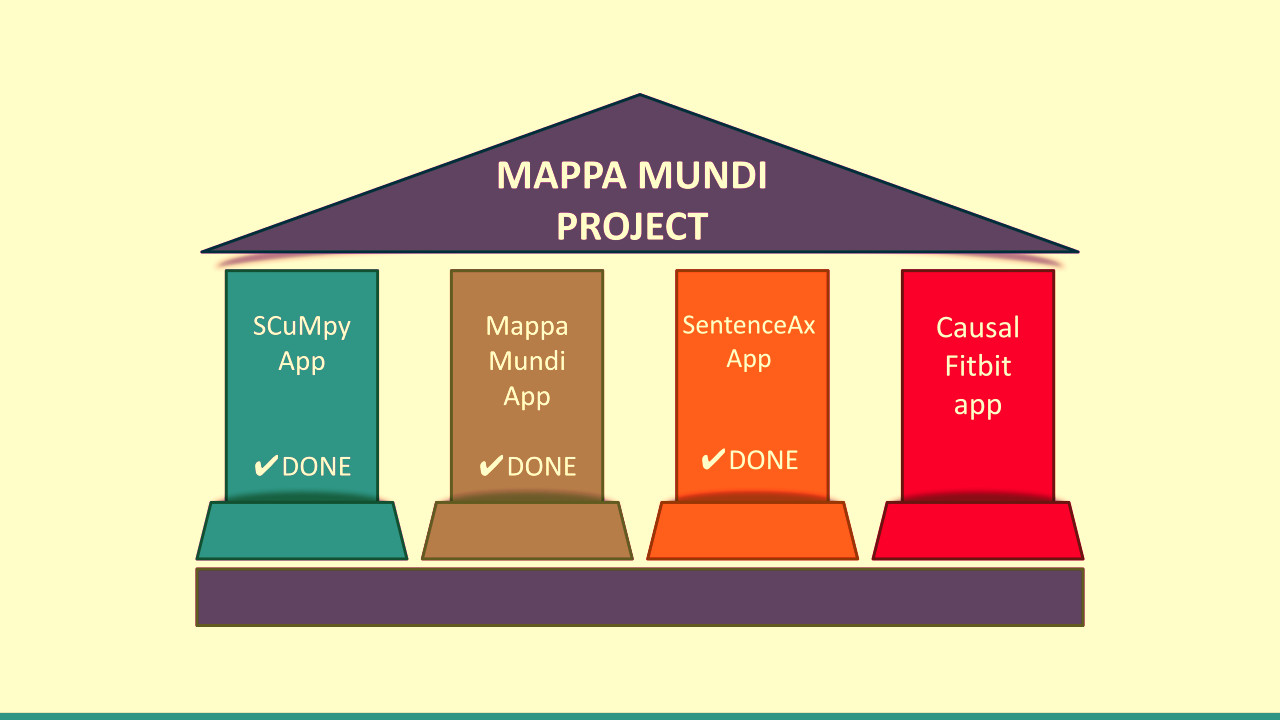
\includegraphics[width=.9\textwidth]{mappa-mundi-4-pillars.jpg
}$$


\end{frame}

\BSSframe{MM: Finding Causal Pathways for diseases}

\begin{wrapfigure}{l}{0.8\textwidth}
   \centering
    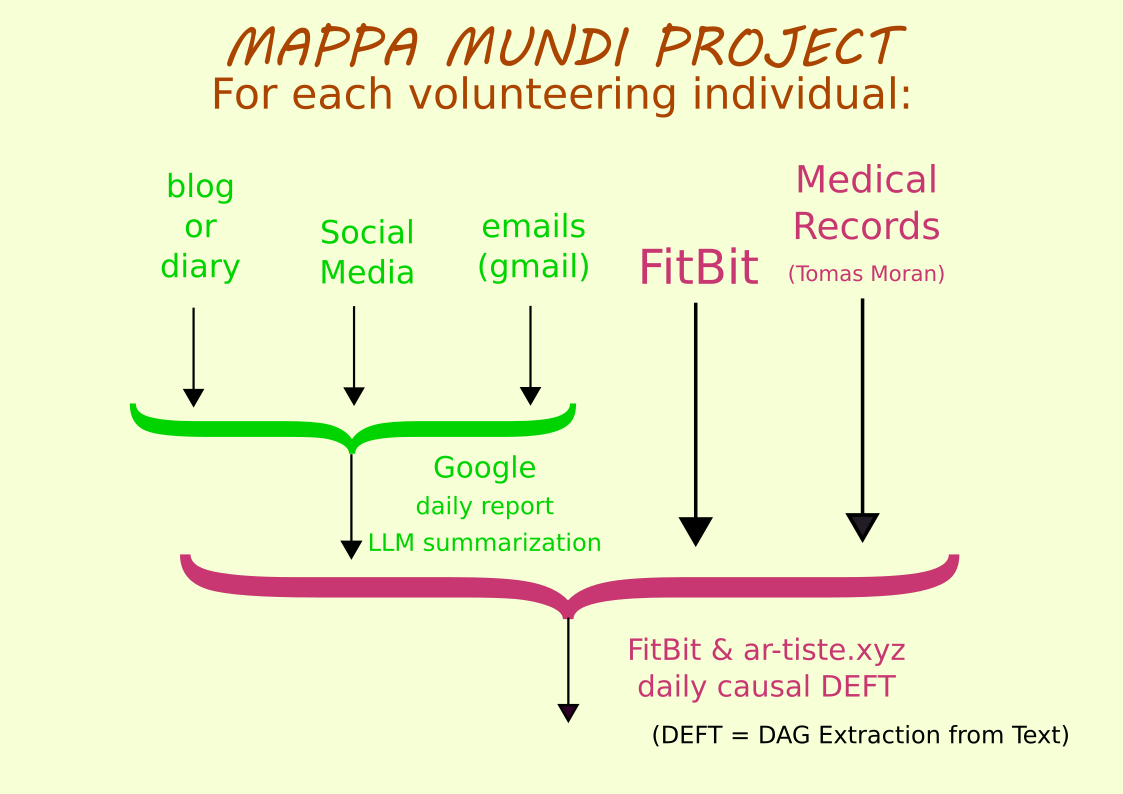
\includegraphics[width=0.8\textwidth]
    {fitbit-artiste.png}

\end{wrapfigure}


How Google can crush its LLM competitors OpenAI and Meta by Bard-ifying its FitBit product line.

\end{frame}






\BSSframe{MM: features}

\begin{itemize}
\item Mappa Mundi (MM) is free open source software that extracts causal networks (DAGs) from text.
\item MM works with any text that does chronological storytelling, such as novels, movie scripts, time stamped lab notebooks and patient diaries. It can be used to find causal pathways to diseases.
\item MM uses 2 types of state of the art (SOTA) LLMs
\begin{enumerate}
  \item Openie6 – for SOTA sentence simplification
  \item sentence transformers – for SOTA sentence similarity
  
 \end{enumerate}
\item MM is immune to hallucinations because 1 and 2 are immune
\item MM is immune to copyright infringement lawsuits because 1 and 2 did not use copyrighted data to train.
\item MM can’t be hacked by prompt injection because it doesn’t use prompts.
\end{itemize}

\end{frame}

\BSframe{Causal Genomics}
\end{frame}

\BSframe{Flood and Drought Anticipatory Action}
\end{frame}

\BSframe{Book: Bayesuvius}
\end{frame}


\end{document}


